\documentclass{llncs}
%\pagestyle{headings} %page numbers
%\usepackage[font=small,labelfont=bf]{caption}


%% Language and font encodings
\usepackage[english]{babel}
\usepackage[utf8x]{inputenc}
\usepackage[T1]{fontenc}
\usepackage[outdir=./]{epstopdf}
\usepackage{bm}
\usepackage{float}

\usepackage[]{xcolor}
%% Sets page size and margins
\usepackage[a4paper,top=3cm,bottom=2cm,left=3cm,right=3cm,marginparwidth=1.75cm]{geometry}

%% Useful packages
%\usepackage{amsmath}
\usepackage{graphicx}
\usepackage{tabu}
\usepackage{array}
\usepackage{tcolorbox}
\usepackage[toc,page]{appendix}

\usepackage[colorinlistoftodos]{todonotes}
\title{Towards semantic-rich word embeddings}
\author{Grzegorz Beringer \and Mateusz Jabłoński \and Piotr Januszewski \and Julian Szymański}
%

 \institute{
Faculty of Electronic Telecommunications and Informatics\\
Gda{\'n}sk University of Technology, Gda{\'n}sk, Poland
}

% (feature abused for this document to repeat the title also on left hand pages)

% the affiliations are given next; don't give your e-mail address
% unless you accept that it will be published
%\institute{Faculty of Electronics,
%Telecommunications and Informatics,
%Gdańsk University of Technology,
%ul. Narutowicza 11/12, 80-952 Gdańsk,
%Poland}

\begin{document}
\maketitle
\begin{abstract}

In recent years, word embeddings have been shown to improve the performance in NLP tasks such as syntactic parsing or sentiment analysis.
While useful, they are problematic in representing ambiguous words with multiple meanings, since they keep a single representation for each word in the vocabulary.
Constructing separate embeddings for meanings of ambiguous words could be useful for solving the Word Sense Disambiguation (WSD) task.

In this work, we present how a word embeddings average-based method can be used to produce semantic-rich meaning embeddings, and how they can be improved with distance optimization techniques.
We also open-source a WSD dataset that was created for the purpose of evaluating methods presented in this research.

\keywords{word embeddings, word sense disambiguation}
\end{abstract}

\section{Introduction}
\label{introduction}

Word embedding methods, that map the vocabulary words to low-dimensional continuous space, have been widely applied to various natural language processing (NLP) problems.
They are commonly used as the input representation of words, replacing high-dimensional one-hot encodings, and have been shown to improve the performance in tasks such as syntactic parsing\cite{parsingGrammars} and sentiment analysis\cite{sentimentAnalysis}.

In word embedding methods, such as word2vec\cite{word2vec} or GloVe\cite{GloVe}, each word in the vocabulary has exactly one representation.
While it is enough for most words, it is problematic for ambiguous words, which can contain more than one meaning.
For example, consider the following examples with the word \textit{tree}, extracted from Wikipedia articles:

\medskip
(a) \textit{The olive, known by the botanical name Olea europaea, meaning "European olive", is a species of small \textbf{tree} in the family Oleaceae [...]}

(b) \textit{Many theories of syntax and grammar illustrate sentence structure using phrase \textbf{trees}, which provide schematics of how the words in a sentence are grouped and relate to each other.}

(c) \textit{Upon completion of listing all files and directories found, \textbf{tree} returns the total number of files and directories listed.}
\medskip

All three sentences mention the word \textit{tree} (or \textit{trees}), but the meaning differs based on context - (a) means tree as a forest plant, (b) tree as a parse tree, (c) tree as a command in Unix systems.

For many applications, such as improving relevance of search engines, anaphora resolution or coherence, identifying which meaning is used, based on context, is important.
This task is called Word Sense Disambiguation (WSD) and is an open problem in NLP domain.
Word embeddings cannot be applied to WSD out-of-the-box, since they cannot differentiate between multiple meanings of an ambiguous word.

In this work, we suggest to create semantically rich embeddings for each meaning of a word (\textit{keyword}) (\ref{sec:kw_embed}), by averaging embeddings of the ambiguous word and words describing its meaning (\ref{sec:baseline_model}).
We evaluate this approach on a small WSD task, gathered from Wikipedia articles (\ref{sec:dataset}).
Word is disambiguated by choosing the closest keyword embedding given the embedding of context, which is an average of word embeddings surrounding the word (\ref{sec:ctx_embed}).
We then propose an optimization method, to improve the quality of embeddings and the result on WSD task as well -  we move keyword embeddings closer to embeddings of contexts they appear in, using examples from the training set (\ref{sec:optimization}).
A number of experiments is run to test the proposed method and its optimized version (\ref{sec:experiments}, \ref{sec:model_analysis}).
Finally, we discuss our findings and present future work (\ref{sec:conclusion}).

\section{Related work}
\label{sec:related_work}

% Word embeddings methods:
%  Latent Semantic Analysis (LSA) and Latent Dirichlet Allocation (LDA)
%  word2vec (skip-gram and CBOW)
%  GloVe
%  fastText?
% WSD background

There have been many methods of creating semantically meaningful word representations.
Global matrix factorization methods, such as latent semantic analysis (LSA)\cite{LSA} use matrix factorization to perform rank reduction on a large term-frequency matrix, that captures statistical information about the corpus.

Local context window methods, like popular skip-gram (SG) or continuous bag-of-words (CBOW) models from word2vec paper\cite{word2vec}, were shown to outperform approaches like LSA at word analogy task.
They use shallow neural networks to either predict context words based on the current word (SG), or predict current word based on context words (CBOW).
FastText\cite{fastText} enriches skip-gram word embeddings, by representing each word as a bag of character n-grams, which also has an added benefit of the ability to compute word representations for words unseen during training.

Global Vectors (GloVe)\cite{GloVe} aim to combine both global matrix factorization and local context window methods, by training on nonzero elements in word-word co-occurence matrix, which leverages global corpus statistics and performs well on word analogy and similarity tasks.

Iacobacci et al.\cite{embeddingsforWSD} were the first to try to use word embeddings for Word Sense Disambiguation.
They consider four different strategies for integrating a pre-trained word embeddings as context representation in a supervised WSD system: concatenation, average, fractional and exponential decay of the vectors of the words surrounding a target word.
Peters et al.\cite{deepcontext} create word representations that differ from traditional word embeddings in that each token is assigned a representation that is a function of the entire input sentence. They use vectors derived from a bidirectional LSTM that is trained with a coupled language model objective on a large text corpus.

The most usual baseline for WSD task is the Most Frequent Sense\cite{evalmfs} (MFS) heuristic, which selects for each target word the most frequent sense in the training data.
Recent growth of sequence learning techniques using artificial neural networks contributed to WSD research: Raganato et al.\cite{neuralseqmodelingforWSD} propose a series of end-to-end neural architectures directly tailored to the task, from bidirectional Long Short-Term Memory (LSTM) to encoder-decoder models.
Melamud et al.\cite{context2vec} also use bidirectional LSTM it their work. They use large plain text corpora to learn a neural model that embeds entire sentential contexts and target words in the same low-dimensional space, which is optimized to reflect inter-dependencies between targets and their entire sentential context as a whole.

%Typically, there are two kinds of approach for Word Sense Disambiguation (WSD): supervised, which make use of sense-annotated training data, and knowledge-based, which make use of the properties of lexical resources.
%In supervised approach, the most widely used training corpus used is SemCor\cite{semcor}, with 226,036 sense annotations from 352 manually annotated documents.
%Knowledge-based systems usually exploit WordNet\cite{wordnet} or BabelNet\cite{babelnet} as semantic network.
%Our solution joins two approaches. We use the knowledge-based word embeddings like GloVe\cite{GloVe} as a baseline for our method and then optimize them in supervised fashion.

%Most of the previous neural networks applications to WSD ignore lexical resources like glosses (sense definitions) and rely solely on word's context. In Luo et al.\cite{glosses} paper, they integrate the context and glosses of the target word into a unified framework, in order to make full use of both labeled data and lexical knowledge.

%Entity Linking (EL) and WSD both address the lexical ambiguity of language. The aim of EL is to discover mentions of entities within text and to link them to the most suitable entry in a reference knowledge base. The two tasks are pretty similar, but they differ fundamentally: in EL the textual mention can be linked to a named entity which may or may not contain the exact mention, while in WSD there is a perfect match between the word form and a suitable word sense in the knowledge base.
%Moro et al.\cite{babelfy} present Babelfy, a unified graph-based approach to EL and WSD based on a loose identification of candidate meanings coupled with a densest subgraph heuristic, which selects high-coherence semantic interpretations.
%We can find also application of random walks\cite{randomwalks} and topic models\cite{topicmodels} for knowledge-based WSD.

%Developing WSD system requires much effort and as a result, very few open source WSD systems are publicly available. Zhong et al.\cite{itmakessense} present an English all-words WSD system, IMS (It Makes Sense), built using a supervised learning approach that is written in Java and completely open source. Following Lee and Ng\cite{SVMtoWSD}, they adopt support vector machines (SVM) as the classifier and integrate multiple knowledge sources including parts-of-speech (POS), surrounding words, and local collocations as features.

\section{Dataset}
\label{sec:dataset}

For the purpose of constructing semantic-rich word embeddings, we manually gathered usage examples for 6 ambiguous words, 4 to 7 meanings each (28 meanings in total) (Table \ref{table:dataset}).
Ambiguous word together with its meaning constitues a \textit{keyword}, which we use as a separate class when identyfing the closest meaning given some context.
All keywords can be seen on Fig. \ref{fig:keywords}.

\begin{table}
\centering
    \begin{tabular}{ | m{7.5cm} | m{1cm} | }
        \hline
        Number of ambiguous words & 6 \\
        \hline
        Number of meanings per ambiguous word & 4 to 7 \\
        \hline
        Number of keywords (ambiguous word + meaning) & 28 \\
    \hline
    \hline
    Number of training examples per keyword & 5 \\
    \hline
    Number of test examples per keyword & 10 \\
    \hline
    \end{tabular}
    \caption{Statistics of the dataset collected for the purpose of this paper. Training examples can be used by the model to optimize semantic-rich word embeddings (Section \ref{sec:optimization}). Test examples are used to evaluate the embeddings and cannot be trained on.}
    \label{table:dataset}
\end{table}

\begin{figure}
    \centering
    \caption{Ambiguous words with their meanings that are present in the dataset. Each word-meaning pair is called a keyword, e.g. \textit{tree (forest)}, \textit{pool (computer science)}.}
    \label{fig:keywords}
    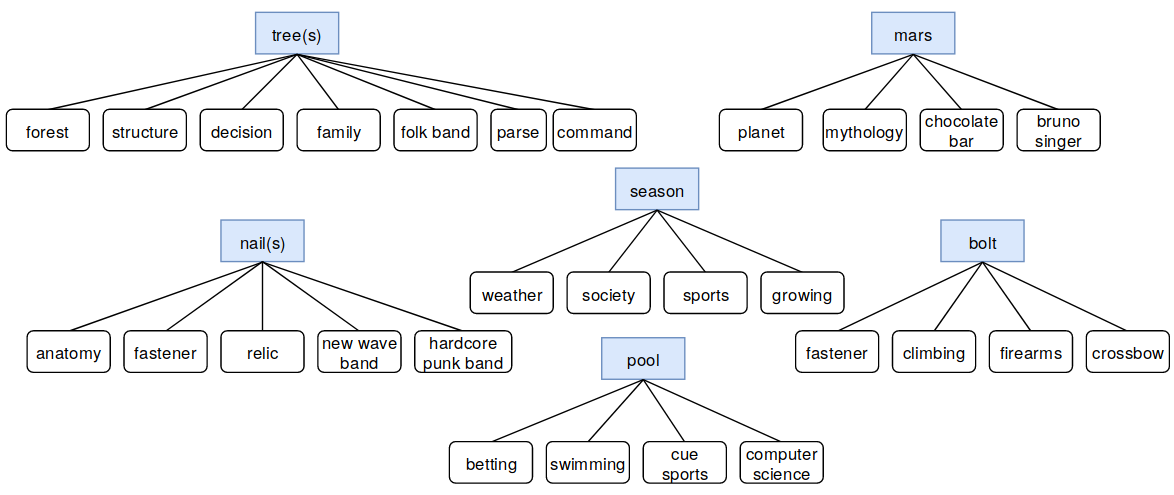
\includegraphics[scale=0.35]{res/keywords.png}
\end{figure}

We chose ambiguous words based on the number and variety of meanings it had.
Meanings themselves were chosen to cover a range of topics (e.g. \textit{tree (forest)}, \textit{tree (family)}, \textit{trees (folk band)}, \textit{tree (command)}).
We also tried to look for meanings that are semantically related and can occur in similar context (and in turn be difficult for the model to differentiate between), e.g. \textit{tree (structure)}, \textit{tree (parse)}, \textit{tree (decision)} or \textit{nails (new wave band)}, \textit{nails (hardcore punk band)}.
Lastly, we added some keywords, that we suspected to be really underrepresented in the word embedding of the ambiguous word, e.g. \textit{Mars} as the pop singer Bruno Mars (\textit{mars (bruno singer)}) or \textit{pool} as the computer science term (\textit{pool (computer science)}).

Usage examples for keywords were gathered mostly from Wikipedia, using \textit{What links here} utility, which lists all Wikipedia pages that link to a specific article.
We used these links to search for usages of our keywords in context.
We found that \textit{What links here} utility has some limitations.
Many articles linked to the keyword do not use that keyword in text at all or just list it in "See also" section, which does not provide good context around the keyword for the model to improve on.
Moreover, some keywords do not have enough usage examples that can be found on Wikipedia alone.
In such cases, other websites were used to find proper usage examples.

The dataset is split into training and test set, with 5 training and 10 test examples for each keyword.
Each example is stored in plain text, with the ambiguous word marked with "*" on both sides.
For simplicity, only one word is marked in each text, even if more ambiguous word usages can be found.
In case we wanted to mark another word in the same text, we could just add the same example twice, with different words marked each time.

The correct keyword for each example, together with a path to file and a link, where the original text was taken from, are stored in CSV files: \textit{train.csv} for training set, \textit{test.csv} for test set (columns: path,keyword,link).
Keywords themselves, together with links to their Wikipedia articles, are stored in \textit{keywords.csv} file (Figure \ref{fig:dataset_format}).

Dataset, together with the code to execute experiments from this paper, can be found on our GitHub repository\footnote{https://github.com/gberinger/automatic-wiki-links}.

\begin{figure}
    \centering
    \caption{Dataset format with an example for \textit{bolt (crossbow)} keyword (highlighted text and arrows). Usage examples are stored in plain text, with ambiguous word marked with "*" (right), and are divided into training and test set. Paths to all test (training) examples can be read from \textit{test.csv} (\textit{train.csv}), together with the links to where they were taken from (middle). All keywords are stored in \textit{keywords.csv}, along with the link to their Wikipedia articles (left).}
    \label{fig:dataset_format}
    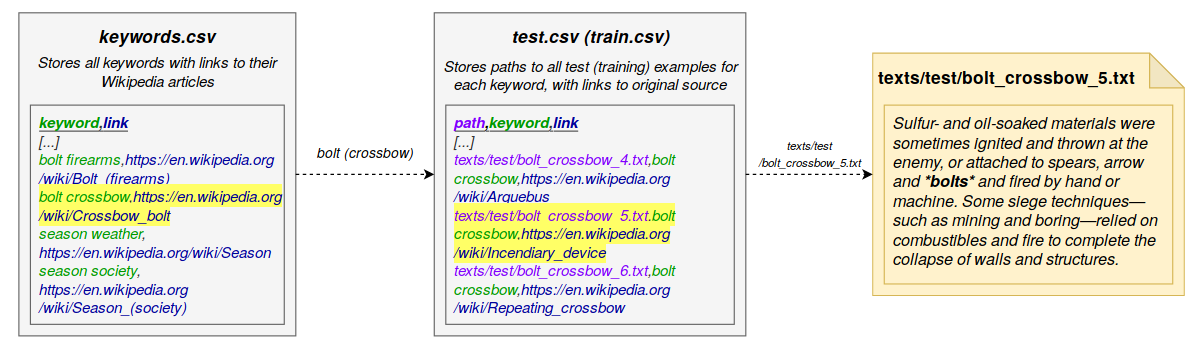
\includegraphics[scale=0.35]{res/dataset_format.png}
\end{figure}


\section{Our method}
\subsection{Keyword embedding}
\label{sec:kw_embed}
\textit{Keyword} is a sequence of words that lets us disambiguate between different meanings of the same ambiguous word, e.g. \textit{tree (forest)} that represents a tree as a plant and \textit{tree (structure)} which represents tree as a mathematical structure.

To get the embedding of the keyword, we average embeddings of all the words in the keyword:

\begin{equation}
    \label{eq:keyword_embedding}
    \bm{k} = e(w_1, w_2, ..., w_N) = \frac{1}{N}\sum_{i=1}^{N} e(w_i)
\end{equation}

where \(e(\cdot)\) is the embedding function used and \(w_1, w_2, ..., w_N\) is a sequence of N words that, in this case, constitutes a keyword.

Example for keyword \textit{tree (forest)}:

\begin{equation}
    \label{eq:example_kw_embed}
    \bm{k}_{tree (forest)} = e(tree, forest) = \frac{e(tree) + e(forest)}{2}
\end{equation}

\subsection{Context embedding}
\label{sec:ctx_embed}
\textit{Context} is a sequence of words that contains an ambiguous word within, usually in the middle.
It is parametrized by \textbf{context length \(l\)}, which specifies how many of words from both side of the ambiguous word in question were taken into consideration.

\textit{Context embedding} \(\bm{c}\) is also achieved by taking an average of word embeddings (Equation \ref{eq:keyword_embedding}).
In this case, \(N = 2l + 1\) and \(w_1, w_2, ..., w_N\) is the context with ambiguous word inside. For some cases \(N < 2l + 1\), since the ambiguous word may occur at the beginning or ending of text example and full context cannot be collected.
In this case, we just average the reduced context.

Text, that we take context from, must be preprocessed.
We remove any special characters and stopwords, and use lower-case letters only. Below is an example taken from the dataset (\ref{sec:dataset}):

\begin{tcolorbox}[
    colframe=blue!25,
    colback=white!10,
    coltitle=white!20!black,
    title={Example for keyword \textit{pool (computer science)} with context length \(l=3\)}]

\textbf{Text}:
\textit{"The object pool pattern is a software creational design pattern that uses a set of initialized objects kept ready to use – a " *pool* " – rather than allocating and destroying them on demand."}

\textbf{Preprocessed text}:
\textit{"the object pool pattern is a software creational design pattern that uses a set of initialized objects kept ready to use a *pool* rather than allocating and destroying them on demand"}

\textbf{Context}:
\textit{kept ready use \underline{pool} rather allocating destroying}

\textbf{Context embedding}:
\(\bm{c} = \frac{e(kept) + e(ready) + e(use) + e(pool) + e(rather) + e(allocating) + e(destroying)}{7}\)

\end{tcolorbox}

\subsection{Baseline model}
\label{sec:baseline_model}
The basic approach is to use keyword (\ref{sec:kw_embed}) and context embeddings (\ref{sec:ctx_embed}) to find the closest keyword given some context, using cosine distance as a metric.

In other words, given an input text and marked ambiguous word within, we extract the context and compute its embedding \(\bm{c}\) (see example in the frame above). The keyword, whose embedding is closest to \(\bm{c}\) w.r.t. cosine distance, is chosen as the ambiguous word's meaning.

We evaluate this model based on top-k accuracy, which checks, if the embedding for correct keyword is among closest \(k\) keyword embeddings (\ref{sec:exp_baseline}).


\subsection{Optimization}
\label{sec:optimization}
We assume, that the performance of the baseline model (\ref{sec:baseline_model}) (and the quality of keyword embeddings) can be improved, if we provide examples of contexts that the specific keyword appears in. To this end, we move keyword embeddings closer to embeddings of contexts they appear in, using examples taken from the training set (\ref{sec:dataset}).

For each training example, we shift the correct keyword embedding by a factor of \(\alpha\), in the direction of the context embedding, which describes said keyword.

\begin{equation}
    \label{eq:alpha_optimization}
    \bm{k}^{(i+1)} = \bm{k}^{(i)} + \alpha(\bm{c} - \bm{k}^{(i)})
\end{equation}

where \(\bm{k}^{(i)}\) is the embedding of the correct keyword at iteration \(i\), \(\bm{c}\) is the context embedding and \(\alpha\) is a scalar that controls the strength of the update.

\smallskip
We try to optimize the system even further, by also moving top-k closest keywords that are incorrect given the same context.

\begin{equation}
    \label{eq:beta_optimization}
    \bm{m}^{(i+1)} = \bm{m}^{(i)} - \beta(\bm{c} - \bm{m}^{(i)})
\end{equation}

where \(\bm{m}^{(i)}\) is the embedding of incorrect keyword at iteration \(i\) and \(\beta\) is a scalar that controls the strength of the update.

Both optimization methods can be seen on Fig. \ref{fig:opt}. The performance of these techniques is evaluated in \ref{sec:exp_alpha} and \ref{sec:exp_beta}.

\begin{figure}
    \centering
    \caption{Optimization. Square is the context embedding \(\bm{c}\), triangles are the closest keyword embeddings, with \(\bm{k}\) being the correct keyword. Without the optimization, the closest keyword embedding w.r.t to context is \(\bm{m}_{1}\), which is incorrect (a). We move the correct keyword embedding in the direction of the context embedding by the factor of \(\alpha\) (Eq. \ref{eq:alpha_optimization}) and the closest \(N\) incorrect keyword embeddings (here \(N=2\)) away from the context embedding by the factor of \(\beta\) (Eq. \ref{eq:beta_optimization}) (b). After optimization, \(\bm{k}\) is the closest keyword (c).}
    \label{fig:opt}
    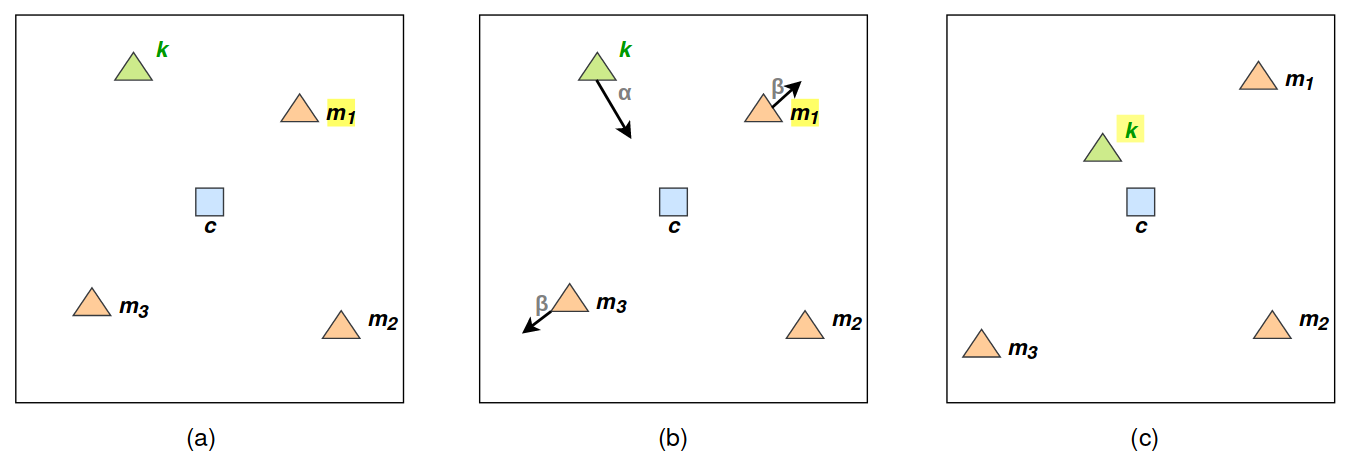
\includegraphics[scale=0.31]{res/opt.png}
\end{figure}


\subsection{Limitations}
\label{sec:limitations}
We are aware that our method has some limitations.
First of all, it may be impossible to achieve the optimal solution, as we can only optimize keyword embeddings, leaving context embeddings fixed in the multidimensional space.
Therefore, it is possible that contexts for specific keyword overlap on contexts for other keyword.

Secondly, the average context embedding may be ambiguous, with a high possibility of two different context being mapped to a similar point in space, especially for longer context legths.
In future work (\ref{sec:conclusion}), we suggest experimenting with different sequence embedding techniques, that might be better suited for this purpose than a flat average.

Finally, we run experiments for a very small number of ambiguous words and meanings (Table \ref{table:dataset}). Our method could have problems with a bigger dataset, since it would be much more difficult to separate different keywords.


\section{Experiments}
\label{sec:experiments}
The goal of following experiments is to check how semantic-rich keyword embeddings (\ref{sec:kw_embed}, \ref{sec:ctx_embed}) perform for the dataset we collected (\ref{sec:dataset}), both for the basic approach (\ref{sec:baseline_model}) and after applying optimization techniques (\ref{sec:optimization}).
We use a pretrained embedding model from spaCy - \textit{en\_vectors\_web\_lg}, which contains 300-dimensional word vectors trained on Common Crawl with GloVe\cite{spacymodel}.

We compare results on the test set with top-k metrics (\(k \in {1, 2, 3}\)), where we check, if the correct keyword is in closest \(k\) keywords given a specific context describing it (\ref{sec:baseline_model}). We focus mostly on top-1 accuracy, since we are interested if the word is correctly disambiguated.

Due to the high impact of training data order on test results, we take the average score of 30 runs (each with a random order of training data) for each optimization experiment.
The best configuration of each experiment is taken as a baseline for the next experiment.
The goal of these experiments is to show how each of parameters influences on model's accuracy after training.

\subsection{Baseline}
\label{sec:exp_baseline}
As the baseline for optimization experiments, we check how keyword and context embeddings perform without any extra optimizations (\ref{sec:baseline_model}).
We evaluate the performance of the baseline model with different context lengths, to see how it affects top-k accuracies (Fig. \ref{fig:baseline}).

\begin{figure}
    \centering
    \caption{Top-k accuracies of the baseline model with different context lengths.}
    \label{fig:baseline}
    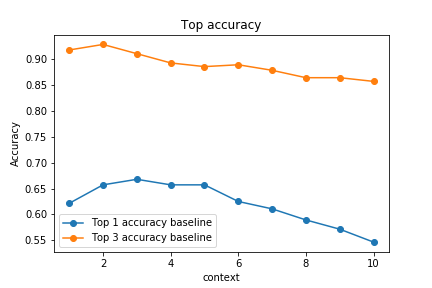
\includegraphics[scale=0.5]{res/baseline_context_top_acc.png}
\end{figure}

We can see, that the model does relatively well, even unoptimized.
Top-3 accuracy is about 85-90\%, which is probably caused by a low number of meanings for each ambiguous word.
Top-1 accuracy for shorter context lengths can go as high as 65\% but decreases with longer contexts.
As suspected (\ref{sec:limitations}), this is most likely due to the fact, that the average of many word embeddings may make some contexts similar to each other, therefore making it harder to distinguish between some meanings.

The best result w.r.t. top-1 accuracy was achieved with \(l=3\), which is why we choose this context length as a starting point for next experiments.

\subsection{Alpha optimization}
\label{sec:exp_alpha}
We check, how an optimization method of moving keyword embeddings closer to the contexts they appear in (Eq. \ref{eq:alpha_optimization}), affects the accuracy of the model.
To do this, we arbitrarily choose some \(\alpha\) value (here 0.2), test the results of improved keyword embeddings with different context lengths and compare them to the baseline (\ref{sec:exp_baseline}). Since we average the results from 30 runs, we mark the measurement uncertainty on the graph (Fig. \ref{fig:exp1_optimization}).

\begin{figure}
    \centering
    \caption{Comparison of the baseline model (\ref{sec:exp_baseline}) and a model optimized with \(\alpha=0.2\) for different context lengths.}
    \label{fig:exp1_optimization}
    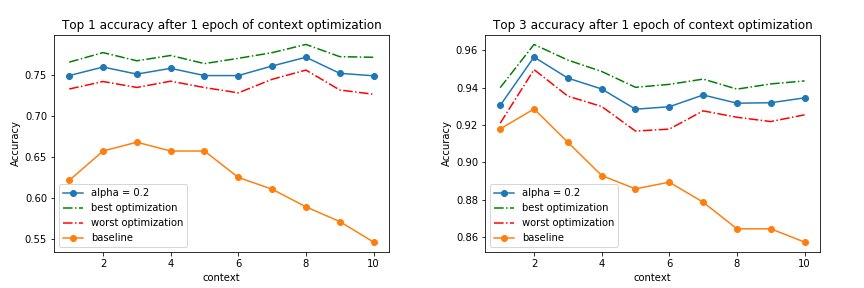
\includegraphics[scale=0.65]{res/exp1_context_top_acc.png}
\end{figure}

Independently of some noise caused by the random order of training data, the optimized model is much better than the base model (12-36\% relative, 10-20\% absolute improvement w.r.t. top-1 accuracy on the test set).
Improvement is most visible for longer context lengths, which achieved relatively poor results in the baseline experiment.
It seems, that a simple optimization may help alleviate the problems with ambiguous embeddings of long contexts (\ref{sec:limitations}).

Overall, results suggest, that for an optimized model, context length is not as important as with the baseline model, at least with this particular \(\alpha\) value.

Next, we check the influence of the \(\alpha\) parameter value on the top-k accuracies for \(l=3\) (Fig. \ref{fig:exp2_alpha}).
Top-1 accuracy improves up to \(\alpha=0.25\) and then starts to drop.
It suggests, that bigger values of \(\alpha\) may cause the movement on the multidimensional plane to be too chaotic, moving the correct keyword embedding too close to a specific context, causing overfitting to a specific example.
Similarly, small values of \(\alpha\) may update the keyword embedding too little, ending up in only slightly better position.

\begin{figure}
    \centering
    \caption{Influence of \(\alpha\) parameter value on top-k accuracies for \(l=3\). Blue line denotes the average result from 30 runs, dotted lines denote worst and best result. The value for \(\alpha=0\) is the result achieved by the baseline model (\ref{sec:exp_baseline}).}
    \label{fig:exp2_alpha}
    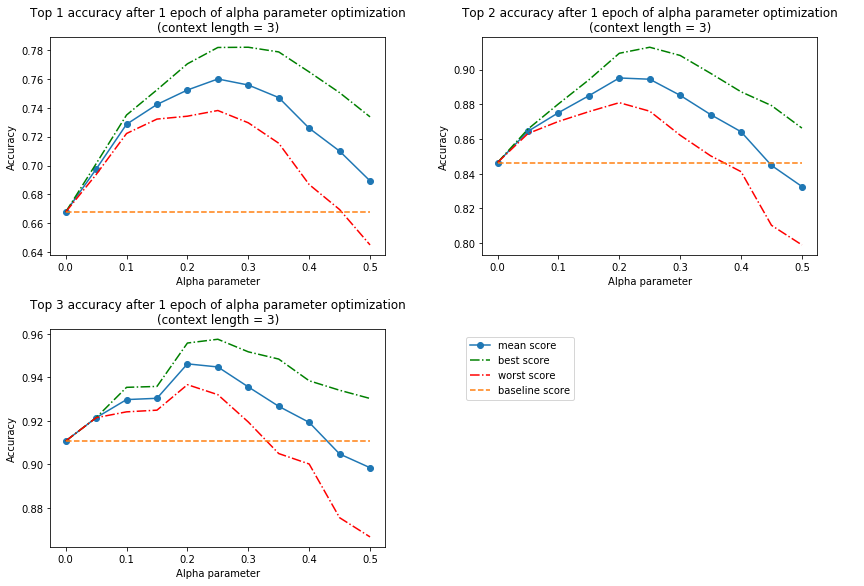
\includegraphics[scale=0.65]{res/exp2_alpha_top_acc.png}
\end{figure}

\subsection{Beta optimization}
\label{sec:exp_beta}
We proved that moving keyword embeddings closer to their contexts is beneficial for the accuracy on the test set (\ref{sec:exp_alpha}).
We assume, that the results could be further improved, if we also increase the distance between closest incorrect keyword embeddings and the context embedding for a specific example (Eq. \ref{eq:beta_optimization}).

In following experiment, we therefore check the influence of \(\beta\) parameter value on the accuracy on the test set, for \(l=3, \alpha=0.25\) (Fig. \ref{fig:exp3_beta}).
Since we compare the results to an average value from previous experiments (Fig. \ref{fig:exp2_alpha}), we decide to only plot an average result achieved by this optimization.

\begin{figure}
    \centering
    \caption{Influence of \(\beta\) parameter value on top-k accuracies for \(l=3\) nad \(\alpha=0.25\). The value for \(\beta=0\) is the best result achieved by the model from previous experiment (Fig. \ref{fig:exp2_alpha}).}
    \label{fig:exp3_beta}
    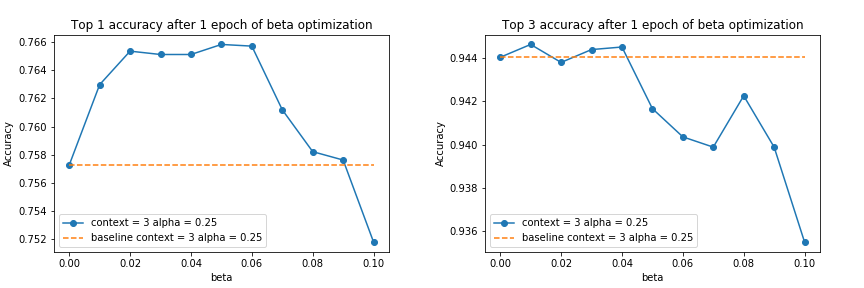
\includegraphics[scale=0.65]{res/exp3_beta_top_acc.png}
\end{figure}

Low values of \(\beta\) seem to slightly improve the performance of our optimization method w.r.t. top-1 accuracy (about 1\% absolute and relative improvement).
High values of \(\beta\) suffer from a similar problem to high values of \(\alpha\), causing too much disruption to keyword embeddings.

We chose to move only top-3 closest keywords per each training example. In future work, it might be interesting to see, how does the number of keyword embeddings moved affects the results. We also theorize, that influence of this particular optimization could be bigger for trainings with more than 1 epoch.

\subsection{Accuracy in training epochs}
\label{sec:exp_epochs}
In previous experiments, we performed only one epoch of training, i.e. we used each training example only once for keyword embeddings optimization.
The goal of this experiment is to check how a number of epochs (full passes through training data) affects the final accuracy.
We run 5 epochs of training, using best parameters from previous experiments: \(l=3, \alpha=0.25, \beta=0.05\) (Fig. \ref{fig:exp4_1_epochs_fixed}).

\begin{figure}
    \centering
    \caption{Top-1 and top-3 accuracy for model with \(l=3, \alpha=0.25, \beta=0.05\) trained for 5 epochs.}
    \label{fig:exp4_1_epochs_fixed}
    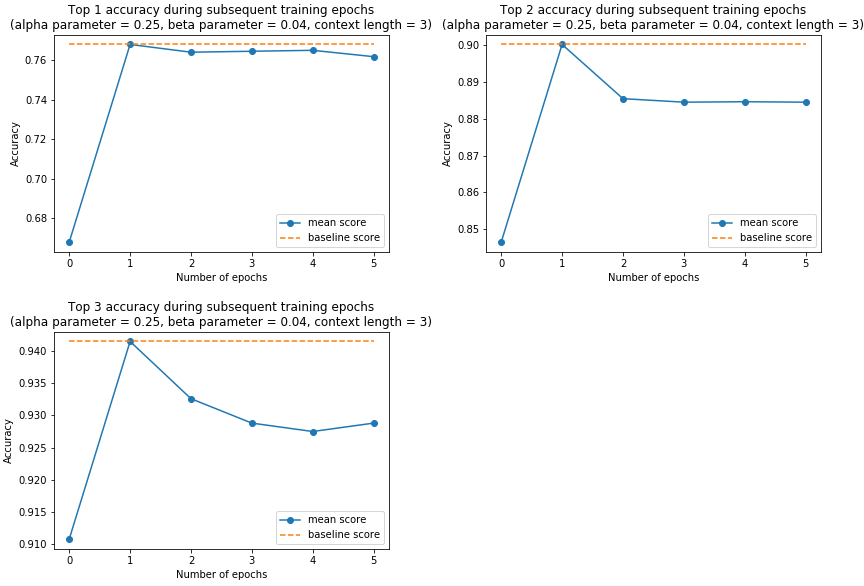
\includegraphics[scale=0.65]{res/exp4_epoch_top_acc.png}
\end{figure}

It can be seen, that there is almost no improvement after the first epoch of training.
The possible problem is that the values of \(\alpha\) and \(\beta\) are too high, causing the updates to keyword embeddings to be too big, similar to what happens, if we choose a big learning rate when training neural networks.
We therefore check what happens, when we choose lower values of these parameters (Fig. \ref{fig:exp4_2_epochs_comparison}).

\begin{figure}
    \centering
    \caption{Comparison of models optimized with different \(\alpha\) and \(\beta\) values with \(l=3\) for 5 epochs.}
    \label{fig:exp4_2_epochs_comparison}
    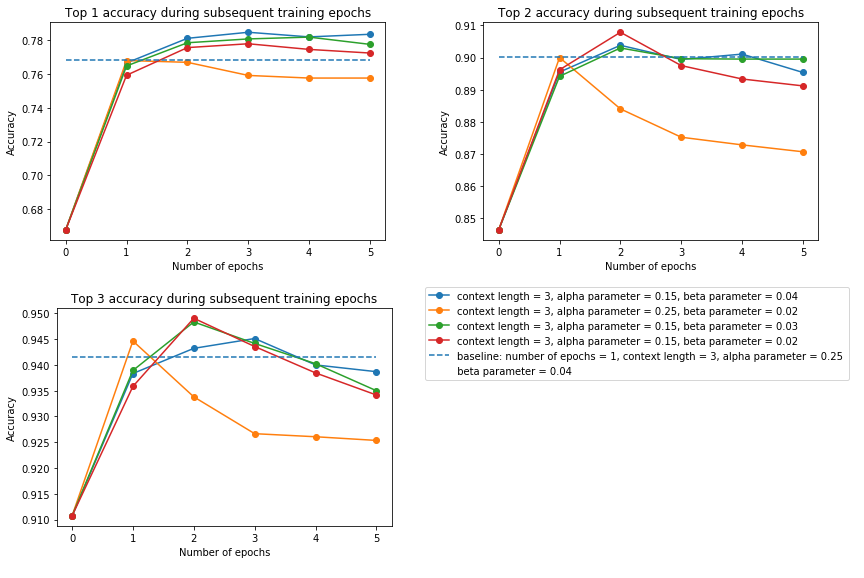
\includegraphics[scale=0.65]{res/exp4_epoch_multiconfiguration_top_acc.png}
\end{figure}

Longer training shows that optimal parameters obtained from previous experiments are not necessarily good for multiple passes through the training data.
If we train for a bigger number of epochs, lower values of \(\alpha\) and \(\beta\) parameters are better.
In future work (\ref{sec:conclusion}) we suggest, that a decay parameter might be useful for this particular reason, with each update being a bit smaller to fine-tune the results.


\section{Model analysis}
\label{sec:model_analysis}
In this section, we take a closer look at how proposed solution performs before (\ref{sec:baseline_model}) and after optimization (\ref{sec:optimization}).
For this purpose, we take a model with context length \(l=4\) as the baseline and then optimize it on the training data (\ref{sec:dataset}) for 4 epochs (\ref{sec:exp_epochs}), using \(\alpha=0.15, \beta=0.04\).

\begin{table}
\centering
\begin{tabular}{ | m{3cm} | m{2cm} | m{2cm} |}
    \hline
    \textbf{Metric} & \textbf{Baseline} & \textbf{Optimized} \\
    \hline
    Avg. cosine distance & 0.348763 & 0.264627 \\
    \hline
    Top-1 accuracy & 66\% & 78\% \\
    \hline
    Top-2 accuracy & 81\% & 90\% \\
    \hline
    Top-3 accuracy & 89\% & 93\% \\
    \hline
\end{tabular}
\caption{Results achieved on the test set for the model before (baseline) and after optimization (4 epochs, \(\alpha=0.15, \beta=0.04\)). Cosine distance is measured between the correct keyword and context embeddings.}
\label{table:model_analysis}
\end{table}

Performance on the test set can be seen in Table \ref{table:model_analysis}.
All metrics improved due to the optimization process of moving correct keywords closer to (and incorrect keywords away from) contexts found in the training set.
High top-2 and top-3 accuracies suggest, that the correct keyword is usually relatively close to the context describing it, even with the baseline model.

For the purpose of analysing which keywords get confused with each other, confusion matrices were constructed for each ambiguous word, for the baseline and optimized model (due to space constraints, Fig. \ref{fig:cm_tree}-\ref{fig:cm_pool} were moved to Appendix \ref{sec:appendix}).
Model was not limited to choosing between the meanings of the specific ambiguous word, but nevertheless, it relatively rarely chose the meaning of unrelated ambiguous word (especially after optimization).
It suggests, that the ambiguous word (which is always a part of context) is usually enough for the context embedding to shift in the direction of meanings connected to this word.

Analysis of confusion matrices also tells us, that some keywords are easier to recognize than other, i.e. the ambiguous word often appears together with its meaning (e.g. \textit{decision tree} or \textit{growing season}, which are coined phrases) or the context in which they appear is often very similar and distinct from the rest (e.g. \textit{tree (command)}).
Moreover, keywords of similar meaning are more likely to get confused, e.g. \textit{nails (new wave band)}, \textit{nails (hardcore punk band)} and \textit{trees (folk band)}, or \textit{tree (decision)}, \textit{tree (structure)} and \textit{tree (parse)}.

It is important to note, that the performance might worsen, if we expand the keyword vocabulary to large-scale experiments, where we have much more possible keywords than 28 (Table \ref{table:dataset}).
We suggest checking the proposed solution on large-scale dataset as possible future work (\ref{sec:conclusion}).


\section{Conclusion and future work}
\label{sec:conclusion}
Constructing semantic-rich embeddings for ambiguous words, by taking the average of embeddings of the ambiguous word and words describing its meaning (\ref{sec:kw_embed}), and then comparing it with the average embedding of context words describing said keyword (\ref{sec:ctx_embed}), proved to be a surprisingly good approach for the task of disambiguation on the dataset of 28 keywords we collected (\ref{sec:dataset}).
The baseline model (\ref{sec:baseline_model}) achieved 67\% top-1, 85\% top-2 and 93\% top-3 accuracy (\ref{sec:exp_baseline}) for context length \(l=3\). Longer context lengths were shown to decrease the accuracy, since the average of many word embeddings may result in similar embeddings for different contexts.

To improve the quality of embeddings, an optimization method of moving keyword embeddings closer to contexts they appear in was suggested (\ref{sec:optimization}).
We have shown, that accuracy on the disambiguation task can be improved up to about 79\% top-1, 90\% top-2 and 95\% top-3 accuracy, even with a few training examples per keyword.
Importance of choosing parameters \(\alpha\) (Eq. \ref{eq:alpha_optimization}) and \(\beta\) (Eq. \ref{eq:beta_optimization}) was shown, with \(\alpha\) being the most crucial for final accuracy (\ref{sec:exp_alpha}).
Moving incorrect keyword embeddings, given some context embedding, controlled by \(\beta\) parameter, was shown to  minimally improve results (\ref{sec:exp_beta}) over only using the \(\alpha\) parameter.
The accuracy was further increased, by performing the optimization over many epochs (i.e. using the training examples more than once, in random order), but with lower values of \(\alpha\) than with a single epoch (\ref{sec:exp_epochs}).

Further improvements could be sought by using different keyword and context embedding schemes, e.g. weighted average or by using some sentence embedding method. Optimization method itself could be made more stable by applying decay to alpha and beta parameters and by using a validation set for early stopping. It could also be bound to cosine distance between the keyword and context - the bigger the difference, the bigger the update.

It would also be interesting to see, how the suggested approach for constructing semantic-rich embeddings would perform on a large-scale dataset.
Such a dataset could be automatically collected from Wikipedia, using disambiguation pages to find ambiguous words and their meanings, and \textit{What links here} utility, to find usage examples for each keyword.

\bibliographystyle{splncs}
\bibliography{sample}

\newpage
\appendix
\section{Appendix}
\label{sec:appendix}

Fig. \ref{fig:cm_tree}-\ref{fig:cm_pool} depict confusion matrices for meanings of ambiguous words, displaying how frequently each keyword was confused with others, before (\ref{sec:baseline_model})(left matrices) and after optimization (\ref{sec:optimization})(right matrices).
Each confusion matrix was limited to meanings of one ambiguous word, with other keywords labeled as \textit{other} on the graph.

Model with context length \(l=4\) was used.  Optimization was done for 4 epochs with \(\alpha=0.15, \beta=0.04\) on the train set. Both baseline and optimized model were evaluated on the test set of 10 usage examples per keyword (\ref{sec:dataset}).

\begin{figure}
    \centering
    \caption{Confusion matrices for \textit{tree} keywords.}
    \label{fig:cm_tree}
    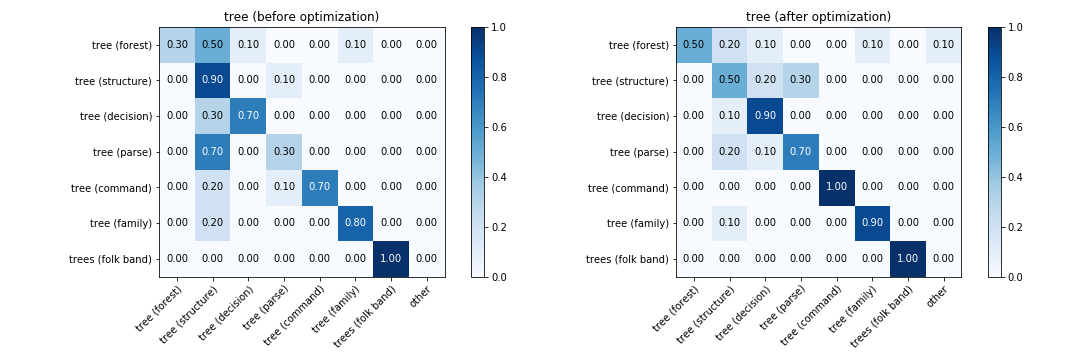
\includegraphics[scale=0.38]{res/cm_tree.png}
\end{figure}

\begin{figure}
    \centering
    \caption{Confusion matrices for \textit{nail} keywords.}
    \label{fig:cm_nail}
    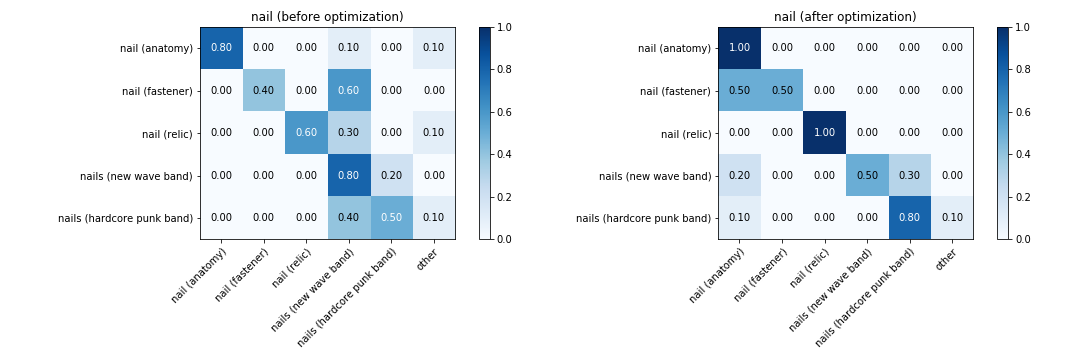
\includegraphics[scale=0.38]{res/cm_nail.png}
\end{figure}

\begin{figure}
    \centering
    \caption{Confusion matrices for \textit{mars} keywords.}
    \label{fig:cm_mars}
    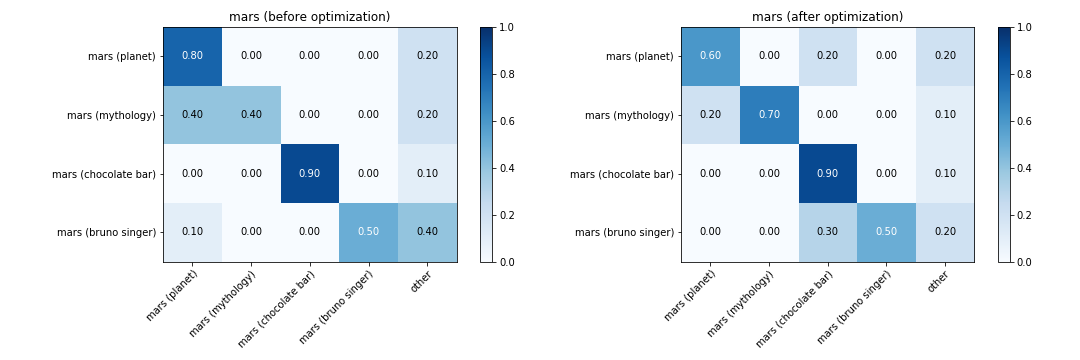
\includegraphics[scale=0.38]{res/cm_mars.png}
\end{figure}

\begin{figure}
    \centering
    \caption{Confusion matrices for \textit{bolt} keywords.}
    \label{fig:cm_bolt}
    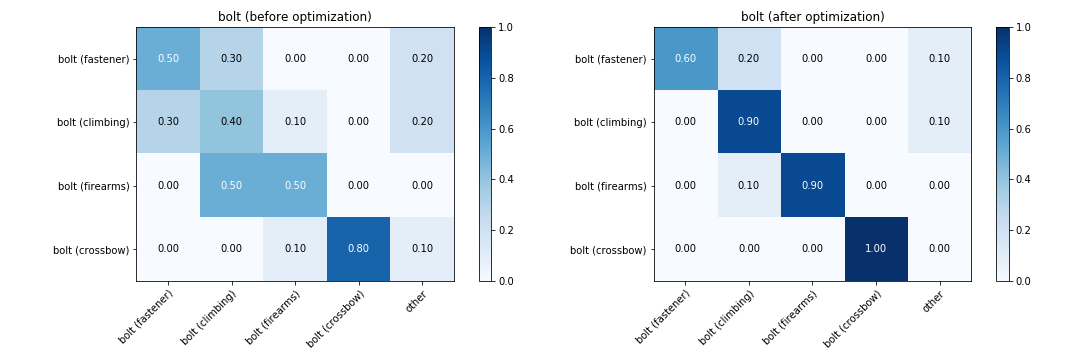
\includegraphics[scale=0.38]{res/cm_bolt.png}
\end{figure}

\begin{figure}
    \centering
    \caption{Confusion matrices for \textit{season} keywords.}
    \label{fig:cm_season}
    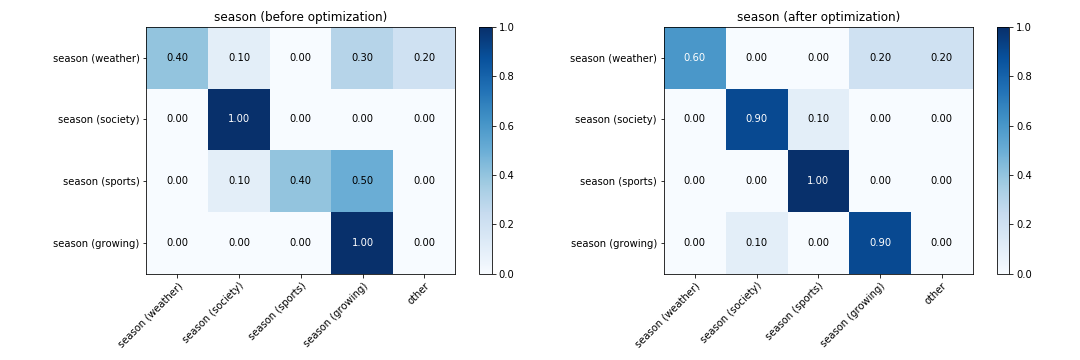
\includegraphics[scale=0.38]{res/cm_season.png}
\end{figure}

\begin{figure}
    \centering
    \caption{Confusion matrices for \textit{pool} keywords.}
    \label{fig:cm_pool}
    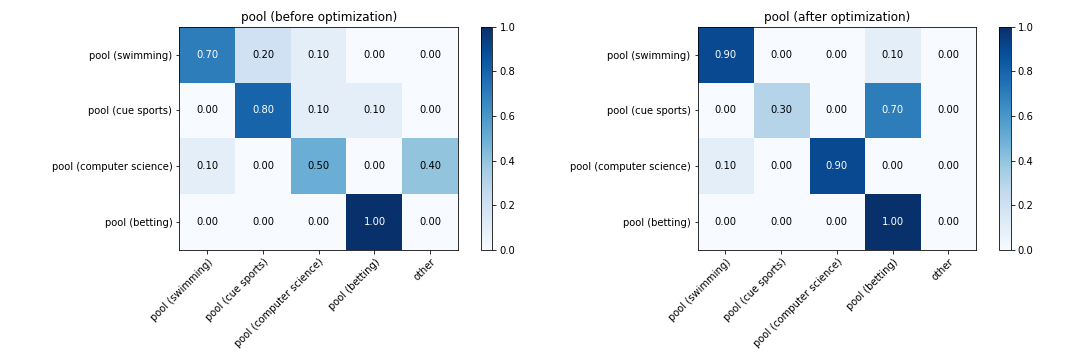
\includegraphics[scale=0.38]{res/cm_pool.png}
\end{figure}

\end{document}


\begin{thebibliography}

\end{thebibliography}
